\section{Gestion des exercices}

\begin{center}
\scalebox{0.7}{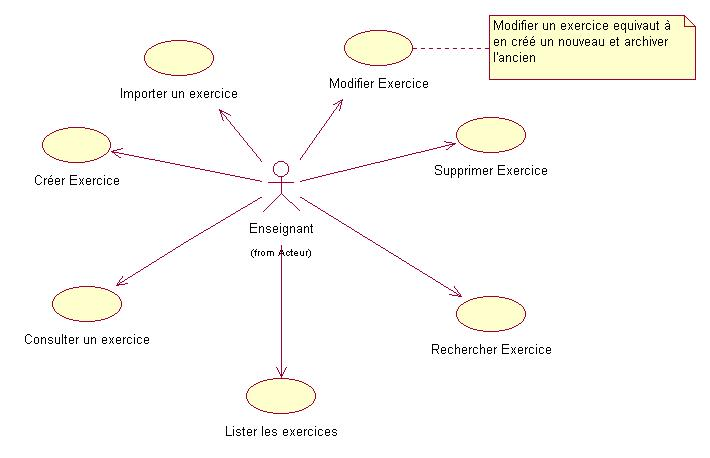
\includegraphics{images/exercice.jpg}}\\
\par{Package Gestion Exercice}
\end{center}
Voici les diff{\'e}rents sc{\'e}narios:\\

\section*{Enseignant}

\begin{tabular}{|p{4cm}|c|p{4cm}|p{5cm}|}
\hline
  Fonction & Priorit{\'e} & Qualit{\'e} & Mesure \\
\hline
Cr{\'e}er un exercice & 1 & Facile et Fiable & Pas de balises {\`a}
  sp{\'e}cifier. Il faut que l'exercice soit tel que le d{\'e}sire
  l'enseignant.\\
\hline
Importer un exercice & 5 & Fiable, rapide & Ne pas g{\'e}n{\'e}rer d'erreur lors du transfert du fichier.\\
\hline
Modifier un exercice & 3 & Suret{\'e} & L'ancien exercice doit {\^e}tre correctement archiv{\'e} pour permettre de revenir en arri{\`e}re.\\
\hline
Supprimer un exercice & 4 & Fiable & L'archivage doit {\^e}tre effectu{\'e} et
  ne pas supprimer l'exercice s'il apparait dans un autre devoir.\\
\hline
Rechercher un exercice & 3 & Rapide & M{\'e}thode d'acc{\`e}s rapide avec mots
  cl{\'e}s.\\
\hline
Lister les exercices & 4 & Clart{\'e} & Permettre d'avoir une vue d'ensemble.\\
\hline
Consulter un exercice & 4 & Rapidit{\'e} et Lisibilit{\'e} & Chargement
  rapide. Affichage clair.\\
\hline
\end{tabular}

\begin{center}
{\'e}chelle de mesure de la priorit{\'e}:

\scalebox{0.5}{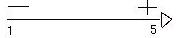
\includegraphics{images/echelle.jpg}}
\end{center}

\begin{itemize}
\item {\bf Cr{\'e}er un exercice :}
	\begin{itemize}
	\item Pr{\'e}-requis : Etre log{\'e}/identifi{\'e}.
	\item Description : L'utilisateur choisit un enseignement.\\
	Il utilise l'{\'e}diteur d'exercice de l'intranet pour cr{\'e}er un exercice.\\
	Il choisit les mots clefs pour l'indexation de cet exercice.
	\item Post-requis : La base des exercices contient un exercice de plus. 
	\end{itemize}

\item  {\bf Importer exercice : }
	\begin{itemize}
	\item Pr{\'e}-requis : Etre log{\'e}/identifi{\'e}.
	\item Description : L'utilisateur choisit un enseignement.\\
	L'utilisateur poss{\`e}de un exercice en XML.
	L'utilisateur importe cet exercice.\\
	Il choisit les mots clefs pour l'indexation de cet exercice.
	\item Post-requis : La base des exercices contient un exercice de plus. 
	\end{itemize}

\item  {\bf Modifier exercice :}
 	\begin{itemize}
	\item Pr{\'e}-requis : Etre log{\'e}/Identifi{\'e}.\\
	L'exercice que l'utilisateur veut modifier existe.
	\item Description : L'utilisateur choisit un exercice.\\
	Il clique l'option {\it Modification}\\
	Il choisit le nouvel exercice 
	\item Post-requis : L'ancien exercice est archiv{\'e}.
	\end{itemize}

\item  {\bf Supprimer exercice :}
	\begin{itemize}
	\item Pr{\'e}-requis : Etre log{\'e}/identifi{\'e}.\\
	L'exercice que l'utilisateur veut supprimer existe.	
	\item Description : L'utilisateur choisit un exercice.\\
	Il clique l'option {\it Suppression}\\
	Une fen{\^e}tre de confirmation apparait.\\
	L'utilisateur confirme son choix.\\
	L'exercice disparait des Tds auxquels il appartenait et est d{\'e}plac{\'e} dans le r{\'e}p{\'e}rtoire d'archives.
	\item Post-requis : L'exercice est supprim{\'e} des Tds et des projets et de la base des exercices.
	\end{itemize}

\item  {\bf Lister exercices :}
	\begin{itemize}
	\item Pr{\'e}-requis : Etre log{\'e}
	\item Description : L'utilisateur choisit un enseignement\\
	L'utilisateur demande le listing des exercices par un simple clique.
	\item Post-requis : La liste des exercices pour un enseignement donn{\'e} est affich{\'e}.
	\end{itemize}


\item  {\bf Rechercher exercice :}
	\begin{itemize}
	\item Pr{\'e}-requis : Etre log{\'e}
	\item Description : L'utilisateur rentre les mots clefs dans un moteur de recherche puis valide son choix.\\
	Une fen{\^e}tre affiche tous les exercices qui contiennent les mots clefs ins{\'e}r{\'e}s.\\
	L'utilisateur peut cliquer sur un lien contenu dans la fen{\^e}tre pour consulter l'exercice de son choix.
	\item Post-requis : L'utilisateur peut choisir parmis les r{\'e}ponses de la recherche.
	\end{itemize}

\item  {\bf Consulter un exercice :}
	\begin{itemize}
	\item Pr{\'e}-requis : Etre log{\'e}
	\item Description : L'utilisateur effectue un listing de tous les exercices ou une recherche.\\
	L'utilisateur choisit l'exercice de son choix.\\
	Il peut consulter l'exercice et les corrections existantes lui correspondants.
	\item Post-requis : L'utilisateur visualise l'exercice choisi.\\
	\end{itemize}
\end{itemize}
